\documentclass[problem]{mcs}

\begin{pcomments}
  \pcomment{PS_product_rule_and_independence}
  \pcomment{by Mike Mekonnen 12/3/11}
\end{pcomments}

\pkeywords{
  product_rule
  independence
  mutual_independence
}

%%%%%%%%%%%%%%%%%%%%%%%%%%%%%%%%%%%%%%%%%%%%%%%%%%%%%%%%%%%%%%%%%%%%%
% Problem starts here
%%%%%%%%%%%%%%%%%%%%%%%%%%%%%%%%%%%%%%%%%%%%%%%%%%%%%%%%%%%%%%%%%%%%%

\begin{problem}
It is possible to have three events $A$, $B$, and $C$ that:

\begin{itemize}
\item satisfy the ``\idx{product rule}.''  That is,
\[
\pr{A \cap B \cap C} = \pr{A} \cdot \pr{B} \cdot \pr{C},
\]

%\item No two out of the three events satisfy the product rule.

\item but are \emph{not} \idx{mutually independent}.
\end{itemize}

\bparts
\ppart Describe a trivial example of this by choosing $A$ with probability zero.

\begin{solution}
If $\pr{A}=0$ then the product rule will hold for any events $B,C$.
So just choose $B,C$ that are not independent to get the required
example.

\end{solution}
\ppart Describe three such events that have nonzero probabilities.

\hint It may be helpful to draw a \idx{Venn diagram} for $\sspace$
containing the three events, and then incrementally fill in the
probabilities of the disjoint regions.

\begin{solution}
One possible answer can be constructed as follows: in the Venn diagram
shown below,
\begin{align*}
\pr{A}  = \pr{B} = \pr{C}  & = x + y\\
\pr{A \cap B} = \pr{A \cap C} = \pr{B \cap C} &  = y\\
\pr{A \cap B \cap C} & = y
\end{align*}

\begin{figure}[h]
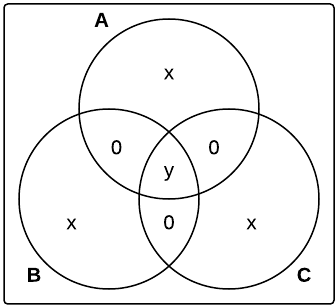
\includegraphics[height=2in]{product-rule-independence-venn}
\end{figure}

With this setup, we need to find nonnegative $x,y$ such that $x+y$ is
positive and
\begin{align*}
\pr{A \cap B \cap C} & = y = (x+y)^3 = \pr{A} \cdot \pr{B} \cdot \pr{C}\\
\pr{A \cup B \cup C} & = 3x + y \le 1.
\end{align*}

We have:
\begin{eqnarray*}
  \pr{A \cap B} &=& y \\
  \pr{A} \cdot \pr{B} &=& (x+y)^2
\end{eqnarray*}

Proving these values unequal shows that $A$ and $B$ are not independent, and so $A$, $B$, and $C$ are not mutually independent.  We must show $y \neq x^2 + 2y + y^2$, which follows from $y < x^2 + 2y + y^2$, or $x^2 + y + y^2 > 0$, which follows from our constraint that $x + y$ is positive (and neither of $x$ nor $y$ is negative). 

Now taking $y = 1/27$ and $x = 8/27$ does the job.

\iffalse
The second requirement is also
satisfied since $3x+y = \frac{25}{27} < 1$.
\fi

Another example is the uniform probability space $[1,10]$ with
\[
 A  \eqdef [1,5],  B \eqdef \set{1,4,5,6,7},  C \eqdef \set{1,3,7,8}.
\]

\end{solution}

\eparts

\end{problem}

%%%%%%%%%%%%%%%%%%%%%%%%%%%%%%%%%%%%%%%%%%%%%%%%%%%%%%%%%%%%%%%%%%%%%
% Problem ends here
%%%%%%%%%%%%%%%%%%%%%%%%%%%%%%%%%%%%%%%%%%%%%%%%%%%%%%%%%%%%%%%%%%%%%

\endinput
